% CHAPTER 1
\chapter{IMPLEMENTATION OF SYNTHETIC INERTIA IN A 9-BUS TEST SYSTEM}
\label{chp:5}
In the Chapter \ref{chp:4}, it is shown that the wind turbine that is connected to grid with back-to-back converter is able to increase its power by almost 0.5pu. Active output power of the turbine can be increased suddenly by utilizing the kinetic energy in the turbine inertia. However, the increase in the fast inertial support is not a function of the grid frequency but a pre-defined period. Nonetheless, the concept of synthetic or virtual inertia suggests a frequency response from renewable energy systems depending on the RoCoF of the electricity grid. As explained at the end of Chapter \ref{chp:3}, a renewable energy system can provide an additional power according to the Swing Equation. \par
In this chapter, the synthetic inertia implementation on a variable speed PMSG wind turbine is tested in P.M. Anderson 9 bus test case which is constructed in Matlab-Simulink environment. Frequency response of the test case is investigated against the sudden load connections in different scenarios. Moreover, the synthetic inertia concept is evaluated in terms of the Turkish electricity network.
\section{P.M.Anderson 9 Bus Test Case}
In order to understand frequency dynamics better, P.M. Anderson test case has been used in the study. P.M. Anderson 9-bus system is one of the test systems in the area of Power Systems to validate the proposed methodologies. It is composed of 9 buses, 3 loads, generators and transformers and 6 lines. IEEE also offers 14, 30 and 118 bus test systems. However, Matlab-Simulink environment restricts the number of buses due to computational burden. This why the 9-bus test system is selected for the synthetic inertia implementation. The single line diagram of the test system is given in Fig. \ref{ieee_9_bus}. The test case consists of three generators and three loads. Generators in the system are connected to 230 kV high voltage (HV) network with step-up transformers.\par
The biggest generator in the system is a hydro power plant with a power rating of 247.5 MVA. The remaining ones are steam generators. The power ratings of the generators are given in Table \ref{generatorproperties}.The loads in the system are connected directly to the HV network. The active and reactive power ratings of the loads are listed in Table \ref{loadproperties}. Detailed system properties are given in Appendix \ref{chp:appendixB}.
\begin{table}[h]
	\centering
	\begin{tabular}{ccc}
		\hline
		\textbf{Generators} & \textbf{Power Rating (MVA)} & \textbf{Plant Type} \\ \hline
		Gen 1               & 247.5                       & Hydro				\\
		Gen 2               & 192                         & Steam               \\
		Gen 3               & 128                         & Steam               \\ \hline
	\end{tabular}
	\caption{Generator Properties of test System}
	\label{generatorproperties}
\end{table}
\begin{figure}[h]
	\centering
	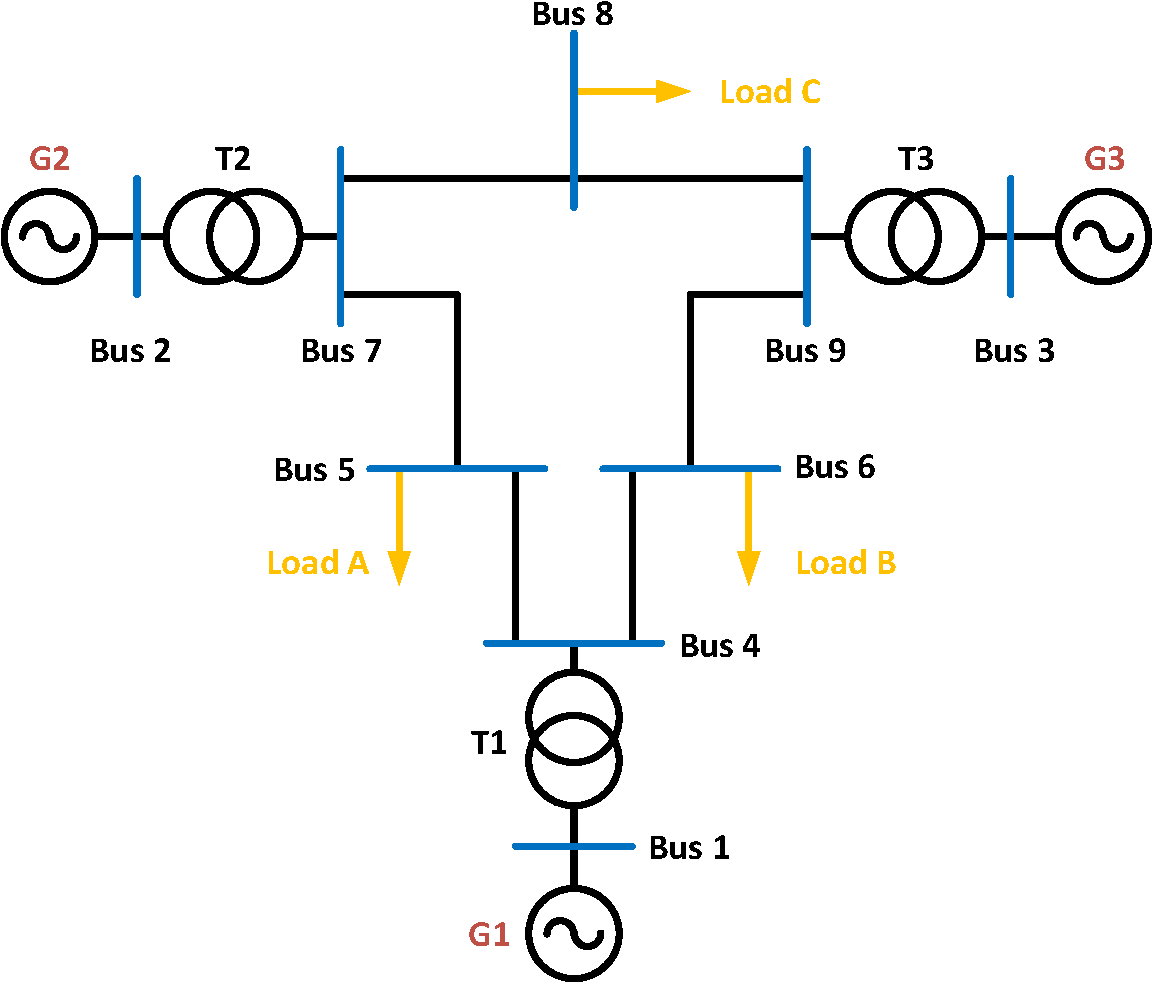
\includegraphics[width=.8\linewidth]{ieee_9_bus.pdf}
	\caption{P.M.Anderson Test Case \cite{P.M.1995}}
	\label{ieee_9_bus}
\end{figure}
\begin{table}[h!]
	\centering
	\begin{tabular}{ccc}
		\hline
		\textbf{Generators} & \textbf{Active Power (MW)}  & \textbf{Reactive Power (MVAr)} \\ \hline
		Load A              & 125                      	  & 50				 \\
		Load B              & 90                          & 30                \\
		Load C              & 100                         & 35                \\ \hline
	\end{tabular}
	\caption{Load Properties of Test System}
	\label{loadproperties}
\end{table}
\subsection{Load Flow Analysis for Base Case}
Successful grid operation requires a load flow analysis in order to ensure that bus voltages are within the allowed band and power flows are below the power carrying capabilities of the lines. In a load flow, system consists of buses whose voltages and phase angles to be calculated. The buses which have a connection with a generator is called as 'PV' bus due to the fact that active power injected to system as well as bus voltage are known before the load flow. Meanwhile, the only load connected buses are called 'PQ' bus with the knowledge of the active and reactive power. For the load flow in the system, one of the buses is selected as slack bus, 'SL' bus with only the voltage is predetermined. The generation of the slack bus will be calculated after the load flow analysis due to the fact that transmission losses in the system are unknown before the analysis. Load flow results are tabulated in Table \ref{loadflow_case1}.
\begin{table}[h!]
	\centering
	\resizebox{\textwidth}{!}
	{
	\begin{tabular}{cclccccc}
		\hline
		Bus \# & Bus Type & \multicolumn{1}{c}{Voltage(pu)} & Angle($^{\circ}$) & Pg(MW)& Qg(MVAr)& Pl(MW)  & Ql(MVAr) \\ \hline
		1      & SL       & \multicolumn{1}{c}{1.04}    & 0     & 71.65 & 27.05  & 0   & 0  \\
		2      & PV       & \multicolumn{1}{c}{1.025}   & 9.28  & 163   & 6.65   & 0   & 0  \\
		3      & PV       & \multicolumn{1}{c}{1.025}   & 4.66  & 85    & -10.86 & 0   & 0  \\
		4      & PQ       & \multicolumn{1}{c}{1.0258}                      & -2.22 & 0     & 0      & 0   & 0  \\
		5      & PQ       & \multicolumn{1}{c}{0.9956}                      & -3.99 & 0     & 0      & 125 & 50 \\
		6      & PQ       & \multicolumn{1}{c}{1.0126}                      & -3.69 & 0     & 0      & 90  & 30 \\
		7      & PQ       & \multicolumn{1}{c}{1.0258}                      & 3.72  & 0     & 0      & 0   & 0  \\
		8      & PQ       & \multicolumn{1}{c}{1.0159}                      & 0.73  & 0     & 0      & 100 & 35 \\
		9      & PQ       & \multicolumn{1}{c}{1.0323}                      & 1.97  & 0     & 0      & 0   & 0  \\ \hline
	\end{tabular}
}
	\caption{Load Flow Results in Base Case}
	\label{loadflow_case1}
\end{table}
\subsection{Base Case Frequency Response for Additional Load Connection}
It is obvious that power system networks experience high RoCoF when either high amount of generation trips or high amount of load is connected to the system. These two main events can be used in the simulation to create frequency disturbances.\par
\begin{table}[h]
	\centering
	\begin{tabular}{ll}
		\hline
		Total System Load                      & 315 MW    \\
		Generator Droop Settings               & 5\%       \\
		Stored Kinetic Energy                  & 3.3 GJ \\
		Effective Kinetic Energy               & 3.3 GJ \\
		Gen 1 Inertia Constant                 & 9.55 s  \\
		Gen 2 Inertia Constant                 & 3.92 s  \\
		Gen 3 Inertia Constant                 & 2.77 s  \\ \hline
	\end{tabular}
	\caption{System Dynamical Properties}
	\label{systemdynamicaldata}
\end{table}
\begin{figure}[h!]
	\centering
	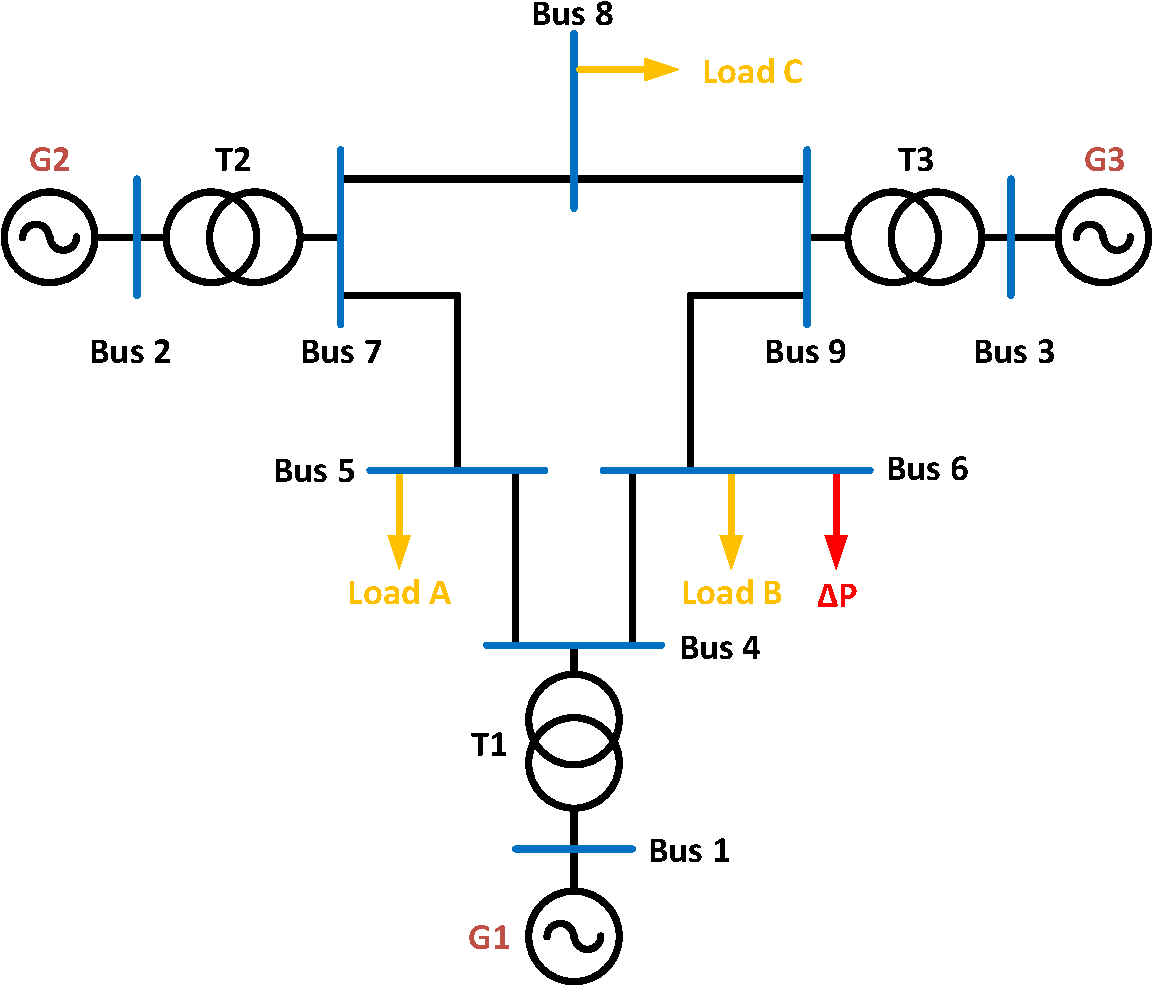
\includegraphics[width=.8\linewidth]{ieee_9_bus_load_position.pdf}
	\caption{Location of the Additional Load}
	\label{ieee_9_bus_load}
\end{figure}
The dynamical properties of the system are listed in Table \ref{systemdynamicaldata}. The system load 315MW is supplied from three conventional generators whose inertia constants varies between 2-9 seconds. Three generators are equipped with governors with 5\% droop settings. Furthermore, the system has 3.3GJ kinetic energy which are effectively supplied from the conventional synchronous generators. \par 
Power generation references are determined based on the load flow of "powergui" toolbox. Machine initialization toolbox is also used to initiate the state of generators in the system. However, the system does not start with the steady state but reaches the steady state within a few seconds. Frequency of the network is disturbed with a load connection when t=10 seconds in order to observe the frequency stability of the system. For 10\% load connection, a load of 31.5MW is connected to system from Bus 6. Location of the additional load is depicted in Fig. \ref{ieee_9_bus_load}.\par
\begin{figure}[h]
	\centering
	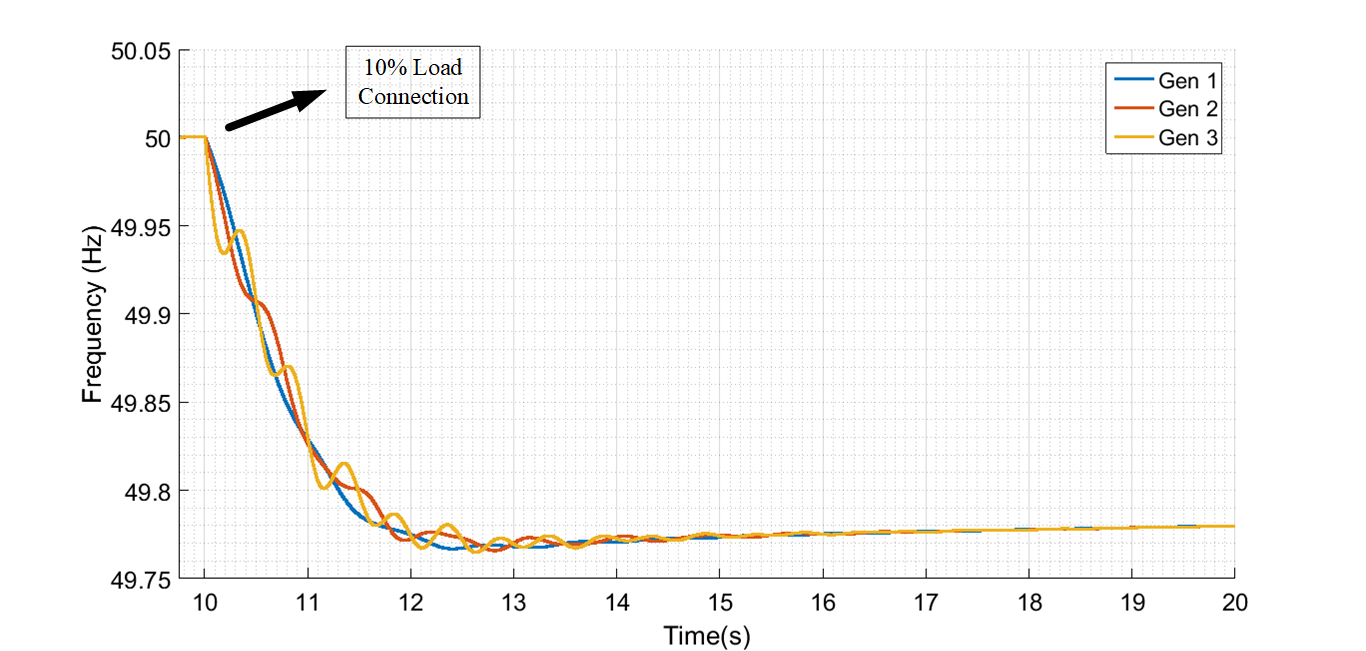
\includegraphics[width=1.0\linewidth]{Case1_Generator_Freqs.png}
	\caption{Generator Frequencies for Frequency Disturbance in Base Case}
	\label{genfreqcase1}
\end{figure}
According to the 10\% load connection to system, generator frequencies are shown in Fig. \ref{genfreqcase1}. As it can be seen from Fig. \ref{genfreqcase1}, rotor swings exists in the frequencies. However, the frequency of generator-1 is the most smooth one due to its huge inertia constant. Meanwhile, the generator-2 and generator-3 follow the frequency of generator-1 with rotor swings.\par
\begin{figure}[h!]
	\centering
	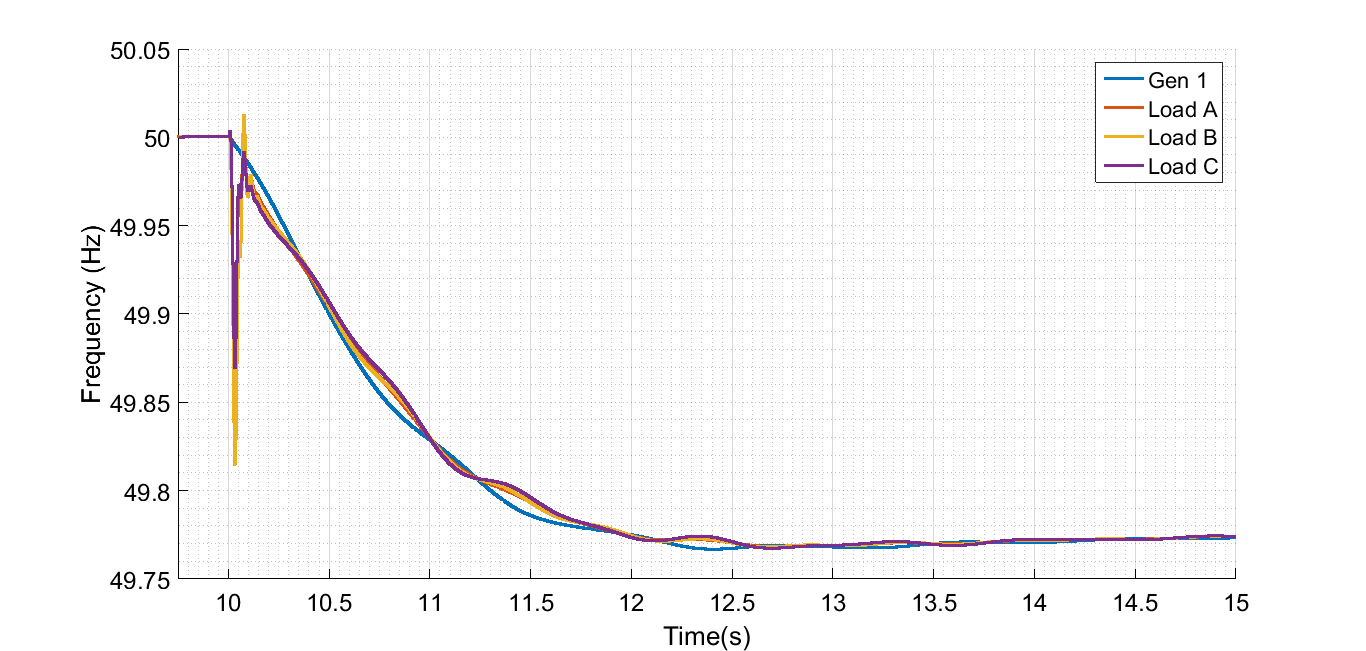
\includegraphics[width=1.0\linewidth]{Case1_Load_Gen_Freqs.png}
	\caption{Frequencies in Generator 1 and Load Buses}
	\label{genfreqcase1_loadgen}
\end{figure}
In the system, the frequencies of loads are almost the same throughout the network since the test system is small enough to assume a single frequency inside the network. This can also be observed in Fig. \ref{genfreqcase1_loadgen} which shows the frequency of the generator-1 as well as the load frequencies captured with PLL (Phase-Locked Loop) block. Another observation is that the load frequencies are also close to the frequency of the generator-1. The only difference is the instant following the load connection. The sharp frequency decline delays the PLL loop to capture the frequency.
\section{10\% Renewable Generation Case}
\label{sec:kmodified}
In order to observe the effect of the renewable energy penetration to the grid, the P.M. Anderson test case is modified such that a wind farm consists of 20 wind turbine is connected to the network. The wind farm has 55MW power rating that consists of 20 of 2.75MW GE2.75-103 model wind turbines. The share of the renewable energy is selected as 10\% of the installed capacity. Moreover, the wind speed is selected as 9m/s that provides 10\% active power generation of the system demand. \par 
Since the transmission network of the test case is under-utilized, the location of the wind farm has no effect on the frequency disturbance. Hence bus 5 is selected as the location for wind farm connection. Modified system is depicted in the Fig. \ref{ieee_9_bus_case2}. In this case, generators 2 and 3 are still assigned to same power generation references. However, the reference generator (generator 1) production is found according to the load flow results. Since the wind turbine also injects power to the transmission network, generator-1 decreases its generation according to the base case.
\begin{figure}[h!]
	\centering
	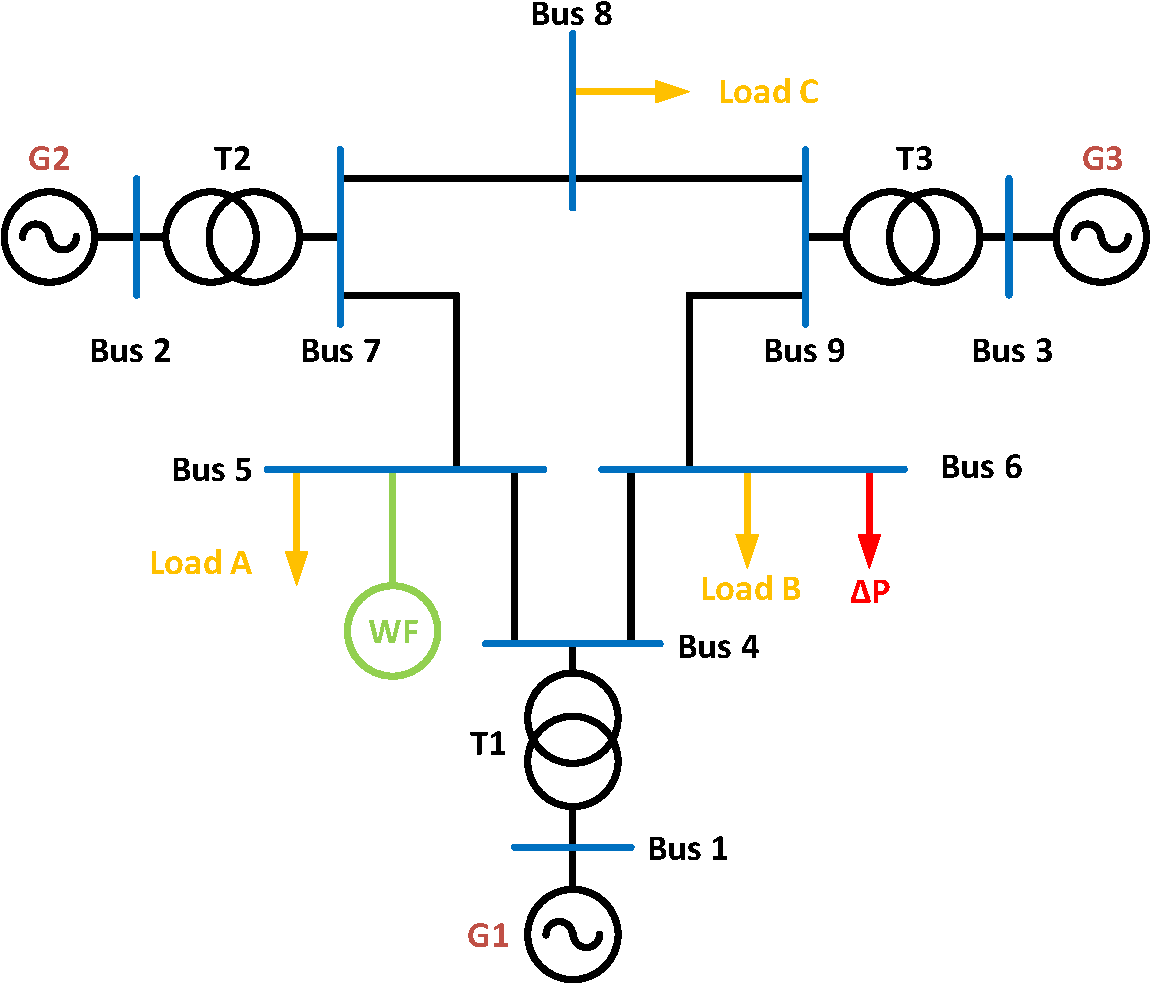
\includegraphics[width=.8\linewidth]{ieee_9_bus_modified.pdf}
	\caption{10\% Renewable Generation Case Single Line Diagram}
	\label{ieee_9_bus_case2}
\end{figure}
\subsection{Load Flow Analysis for 10\% Renewable Generation Case}
Load flow analysis for the modified case is listed in Table \ref{loadflow_case2}. The power injected from Bus 1 is decreased as expected. This can also be seen from the phase angle between buses 1 and 4 which decreased from $2.22^{\circ}$ to $1.18^{\circ}$. Total power generation from active power from conventional generation units are also decreased. Therefore, the modified system resembles the base case with low power demand. The wind farm production cannot be shown in the Bus-5 power generation section since the corresponding bus is a PQ bus. Therefore, the wind farm power is shown in the load side as negative injection to the system. Wind farm produces 35.7MW active power at unity power factor. 
\begin{table}[h!]
	\centering
	\resizebox{\textwidth}{!}
	{
	\begin{tabular}{cclccccc}
		\hline
		Bus \# & Bus Type & \multicolumn{1}{c}{Voltage(pu)} & Angle($^{\circ}$)& Pg(MW)    & Qg(MVAr)     & Pl(MW)  & Ql(MVAr)   \\ \hline
		1      & SL       & \multicolumn{1}{c}{1.04}    & 0     & 38.06 & 25.07  & 0   & 0  \\
		2      & PV       & \multicolumn{1}{c}{1.025}   & 11.33 & 163   & 6.65   & 0   & 0  \\
		3      & PV       & \multicolumn{1}{c}{1.025}   & 6.32  & 85    & -10.86 & 0   & 0  \\
		4      & PQ       & \multicolumn{1}{c}{1.0263}  & -1.18 & 0     & 0      & 0   & 0  \\
		5      & PQ       & \multicolumn{1}{c}{0.9995}  & -1.54 & 0     & 0      & 125-(35.7) & 50-(0) \\
		6      & PQ       & \multicolumn{1}{c}{1.0128}  & -2.43 & 0     & 0      & 90  & 30 \\
		7      & PQ       & \multicolumn{1}{c}{1.0266}  & 5.77  & 0     & 0      & 0   & 0  \\
		8      & PQ       & \multicolumn{1}{c}{1.0164}  & 2.62  & 0     & 0      & 100 & 35 \\
		9      & PQ       & \multicolumn{1}{c}{1.0326}  & 3.62  & 0     & 0      & 0   & 0  \\ \hline
	\end{tabular}
	}
	\caption{Load Flow Results for Modified Case}
	\label{loadflow_case2}
\end{table}
\subsection{10\% Renewable Case Frequency Response for Additional Load Connection}
10\% Renewable Case is very similar to the Base Case except for a wind farm located in Bus 5. The wind farm consisting of 20 turbines also has stored kinetic energy depending on generator speed. Wind speed of 9m/s stores 293.7MJ kinetic energy in the wind farm. By considering this stored energy, dynamical properties of the system is updated in the Table \ref{systemdynamicaldatamod}. Nonetheless, the effective kinetic energy is unchanged in the system due to the fact that rotor frequency is decoupled from grid frequency in the existing wind turbine model.\par
\begin{table}[h]
	\centering
	\begin{tabular}{ll}
		\hline
		Total System Load                      & 315 MW    \\
		Generator Droop Settings               & 5\%       \\
		Stored Kinetic Energy                  & 3.6 GJ \\
		Effective Kinetic Energy               & 3.3 GJ \\
		Gen 1 Inertia Constant                 & 9.55 s  \\
		Gen 2 Inertia Constant                 & 3.92 s  \\
		Gen 3 Inertia Constant                 & 2.77 s  \\ \hline
	\end{tabular}
	\caption{System Dynamical Properties with Wind Farm}
	\label{systemdynamicaldatamod}
\end{table}
The renewable energy system in this case can be considered as a negative load of 35.7MW. Therefore, base case with decreased load is under discussion in this subsection. 10\% additional load (31.5MW) is connected to Bus 6 and the frequency response of the 10\% Renewable Case is shown in Fig. \ref{Case1_2_freq}. \par
\begin{figure}[h]
	\centering
		\begin{subfigure}{0.9\textwidth} % width of right  
			\centering
		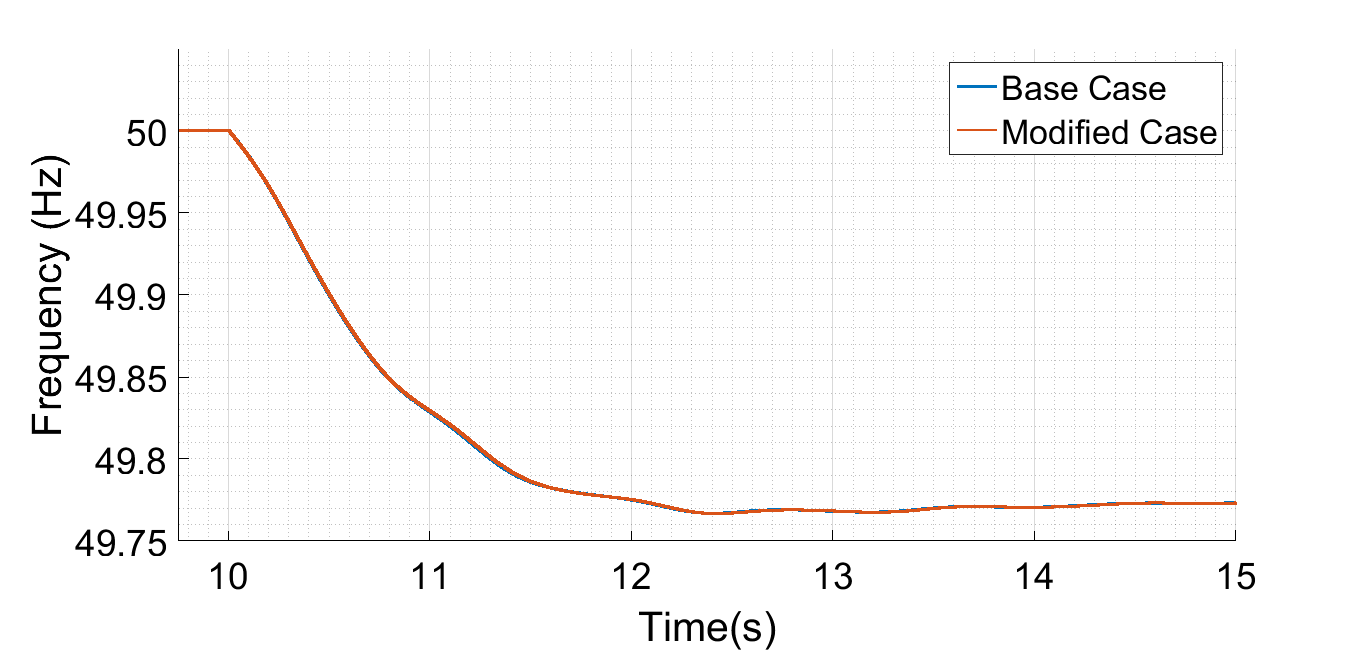
\includegraphics[width=0.9\linewidth]{Case1_2_3.png}
		\caption{Comparison of Frequencies}		
		\label{Case1_2_freq}
		\end{subfigure}
		\vspace{0.1em} % here you can insert horizontal or vertical space
	\begin{subfigure}{0.9\textwidth}
\centering	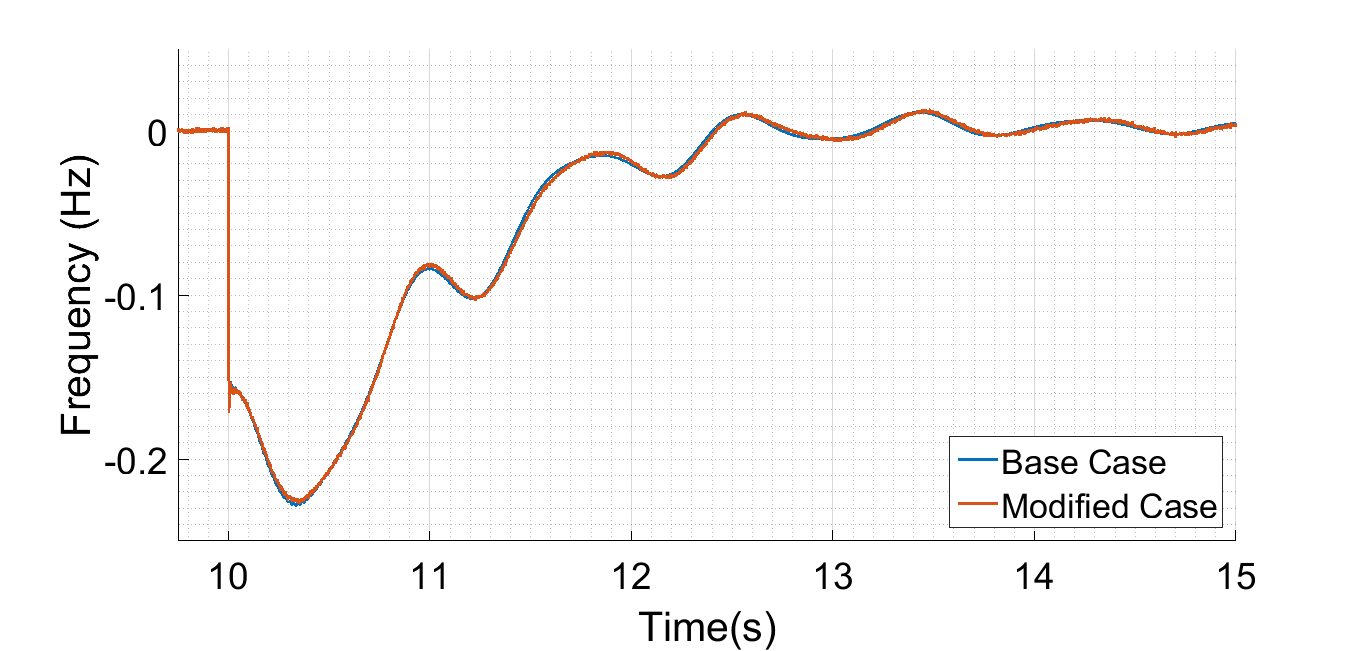
\includegraphics[width=0.9\linewidth]{Case1_2_rocof_3.png}
	\caption{Comparison of RoCoFs}
	\label{Case1_2_rocof}	
	\end{subfigure}
	\caption{Comparison of Base Case and 10\% Renewable Generation Case}
\end{figure}
Almost the same frequency response is observed in the system, as both systems have the same amount of stored kinetic energy. Another reason is that there is no congestion in the system due to under-utilized of transmission network. The same frequency response can also be observed in the rate of change of frequencies in Fig. \ref{Case1_2_rocof}. This concludes that renewable energy penetration does not change the frequency response of the system if the only change in the system is the inclusion of renewable energy system. In other words, renewable energy systems does not affect the frequency response of the grid unless the system is preferred over a conventional generation unit. \par
Notice that the renewable energy systems are intermittent energy sources. Nonetheless, the wind speed is assumed as constant in this study. Assuming constant wind speed is not a disadvantage since the inertial support is based on the kinetic energy of the wind turbine. The variation of the wind speed during the support period affects only the speed recovery process. 
\section{Reduced Inertia Case}
\label{sec:kdecommissioned}
As seen in the \%10 Renewable Generation Case, the frequency response of the system does not change with renewable energy inclusion. However, it is inevitable that renewable energy systems will replace the conventional units in the future. The economic dispatch determines the power plant generation levels according to their energy prices. Since the thermal units have fuel costs compared to wind and solar systems, they might be shut down consequently. In order to investigate the effect of thermal decommissioning, the smallest generator, generator-3, is shut down. When the generator-3 is out of service, the effective inertia decreases by \%10. The reduced inertia case diagram is shown in Fig. \ref{decommissioned_case}.\par
\begin{figure}[h!]
	\centering
	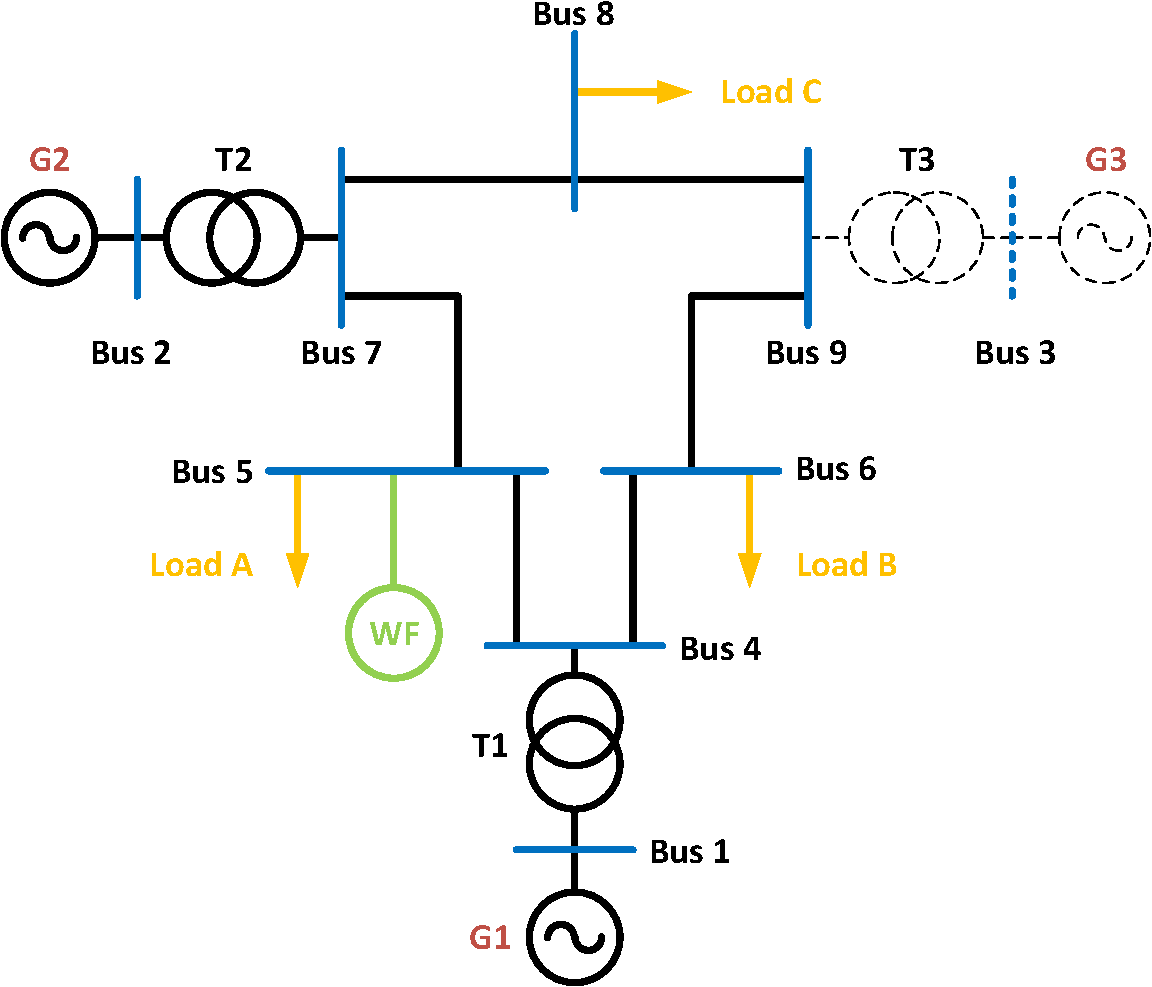
\includegraphics[width=.8\linewidth]{ieee_9_bus_decommissioned.pdf}
	\caption{Reduced Inertia Case Single Line Diagram}
	\label{decommissioned_case}
\end{figure}
\begin{table}[h]
	\centering
	\begin{tabular}{ll}
		\hline
		Total System Load                      & 315 MW    \\
		Generator Droop Settings               & 5\%       \\
		Stored Kinetic Energy 				   & 3.3 GJ \\
		Effective Kinetic Energy 			   & 3.0 GJ \\
		Gen 1 Inertia Constant                 & 9.55 s  \\
		Gen 2 Inertia Constant                 & 3.92 s  \\
		\hline
	\end{tabular}
	\caption{Reduced Inertia Case Dynamical Properties}
	\label{systemdynamicaldatacase3}
\end{table}
Since the generator-3 is out of service, the stored kinetic energy is decreased in the system. Dynamical properties of the reduced inertia case are updated and given in Table \ref{systemdynamicaldatacase3}. Higher RoCoF value and lower frequency nadir are expected with the same additional load since the system dynamical properties are deteriorated with the removal of generator-3.
\subsection{Load Flow Analysis for Reduced Inertia Case}
In this case, the same active power reference (163MW) is again assigned to generator-2. Besides, the wind farm generates active power, 35.7MW at unity power factor. Since the generator-3 is out of service, generator-1 loading is increased. Load flow analysis for reduced inertia case is given in Table \ref{loadflow_case3}.
\begin{table}[h!]
	\centering
	\resizebox{\textwidth}{!}
	{
	\begin{tabular}{cclccccc}
		\hline
		Bus \# & Bus Type & \multicolumn{1}{c}{Voltage(pu)} & Angle($^{\circ}$)& Pg(MW)    & Qg(MVAr)     & Pl(MW)  & Ql(MVAr)   \\ \hline
		1      & SL       & \multicolumn{1}{c}{1.04}    & 0     & 121.76& 16.26  & 0   & 0  \\
		2      & PV       & \multicolumn{1}{c}{1.025}   & 4.18  & 163   & 0.65   & 0   & 0  \\
		4      & PQ       & \multicolumn{1}{c}{1.0332}                      & -3.74 & 0     & 0      & 0   & 0  \\
		5      & PQ       & \multicolumn{1}{c}{1.0083}                      & -5.63 & 0     & 0      & 125-(35.7) & 50-(0)\\
		6      & PQ       & \multicolumn{1}{c}{1.0224}                      & -7.65 & 0     & 0      & 90  & 30 \\
		7      & PQ       & \multicolumn{1}{c}{1.0294}                      & -1.36 & 0     & 0      & 0   & 0  \\
		8      & PQ       & \multicolumn{1}{c}{1.0207}                      & -5.82 & 0     & 0      & 100 & 35 \\
 \hline
	\end{tabular}
}
	\caption{Load Flow Results for Reduced Inertia Case}
	\label{loadflow_case3}
\end{table}
\subsection{Reduced Inertia Case Frequency Response for Additional Load Connection}
Decommissioned system is also subjected to the same frequency disturbance which is the additional load connection from Bus 6. System frequency response is observed and compared to Base Case and Modified Case in Fig. \ref{Case1_2_3_freq}. The frequency response of the system gets worse with the generator 3 decommissioned. It results that the frequency nadir is decreased from 49.77Hz to 49.65Hz due to the decrease in the stored kinetic energy in the system. The deteriorated frequency response can also be seen from the comparison of RoCoFs that is given in Fig. \ref{Case1_2_3_rocof}. 
\begin{figure}[h!]
	\centering
	\begin{subfigure}{0.8\textwidth} % width of right subfigure
	\centering	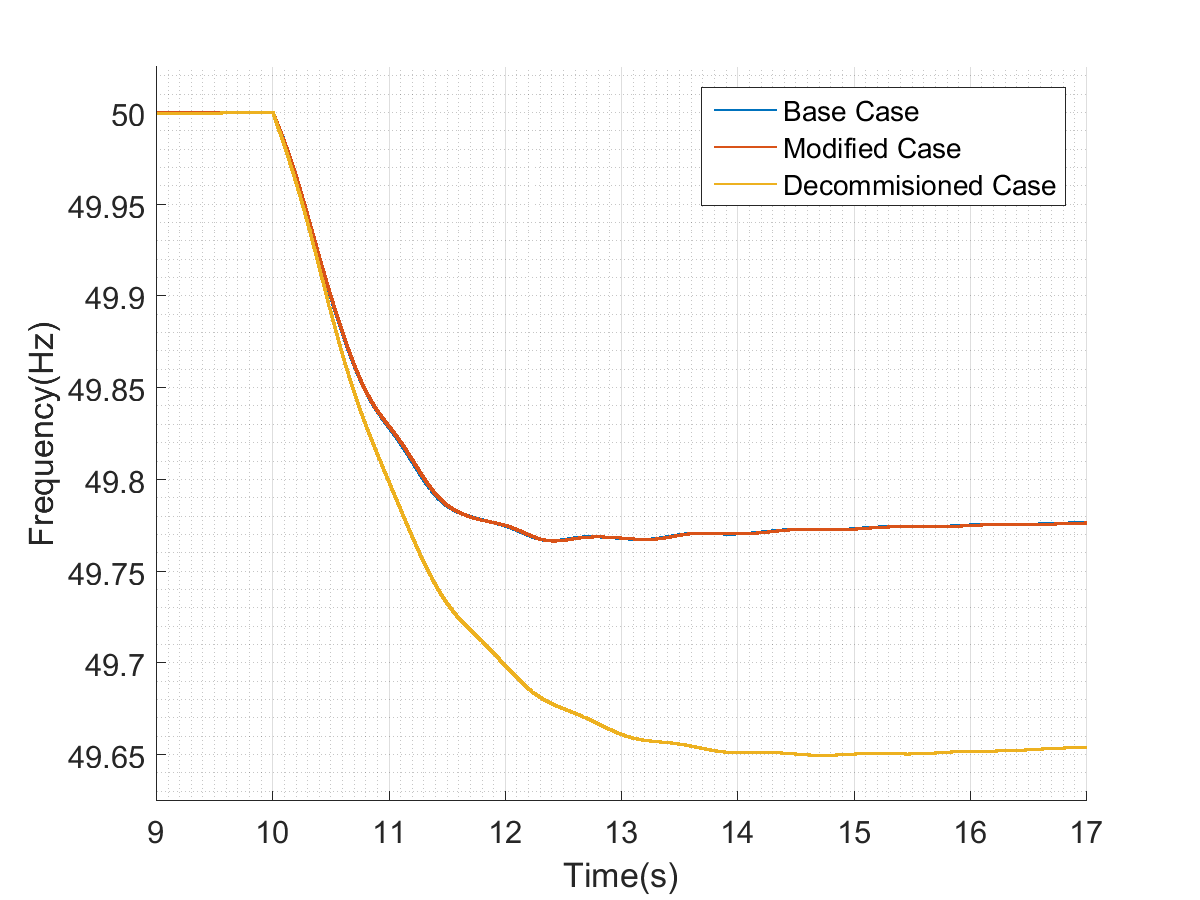
\includegraphics[width=0.8\linewidth]{Case1_2_3_freq.png}
		\caption{Comparison of Frequencies}		
		\label{Case1_2_3_freq}
	\end{subfigure}
	\vspace{0.1em} % here you can insert horizontal or vertical space
	\begin{subfigure}{0.8\textwidth}
	\centering	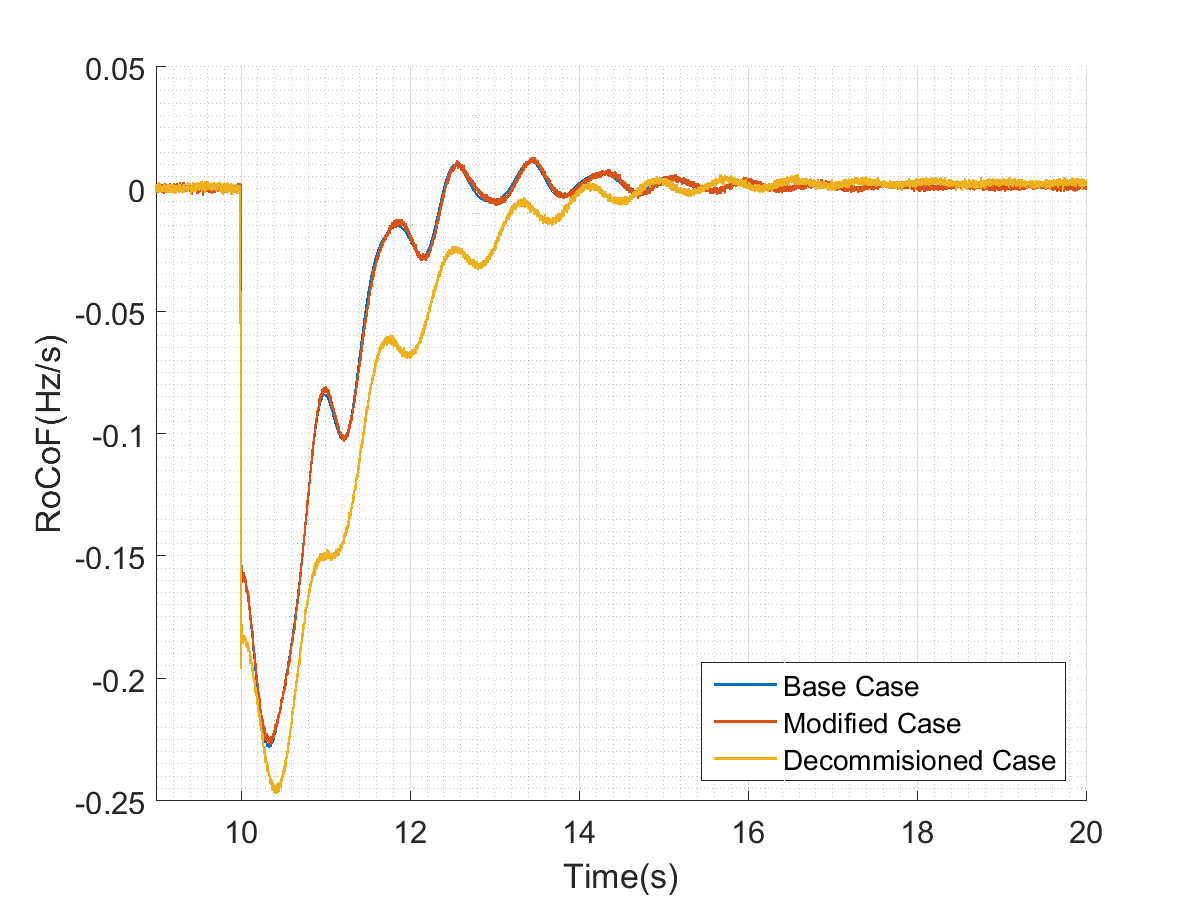
\includegraphics[width=0.8\linewidth]{Case1_2_3_rocof.png}
		\caption{Comparison of RoCoFs}
		\label{Case1_2_3_rocof}	
	\end{subfigure}
	\caption{Comparison of Base Case, \%10 Renewable Case (Modified Case) and Reduced Inertia Case (Decommissioned Case)}
\end{figure}
\section{\%10 Renewable Generation Case with Synthetic Inertia}
The frequency response of the \%10 renewable generation case is investigated in Section \ref{sec:kmodified} and the system frequency was almost the same with test system base case. However, the response of the system can be improved by provision of synthetic inertia. By utilizing the inertial support in the wind turbines, the effective kinetic inertia of the system can be increased. To achieve this purpose, the active powers of the wind turbines are increased according to the grid RoCoF. \par
\begin{equation}
\label{hmax}
2H_{max,med}\overline{f}_{max}\frac{d\overline{f}_{max}}{dt}=\Delta\overline{P}_{e,max}
\end{equation}
\begin{equation}
\label{hmax1}
2H_{max,med}\frac{0.25}{50}=\frac{1}{3.04}
\end{equation}
\begin{equation}
\label{hmax2}
H_{max,med}=32.9s
\end{equation}
Chapter \ref{chp:4} estimates the turbine capability for inertial support depending on the wind speed in the site. Since the wind speed is selected as 9m/s for all turbines in the farm, each wind turbine is able to increase its active power by 1MW according to the Section \ref{sec:klimit}. According to the maximum increase 1MW in the active power and the worst case RoCoF 0.25H/s, maximum inertia constant which can be emulated in the wind speed 9m/s is calculated in Eq. (\ref{hmax2}). However, the increase in the high speed limits the maximum inertia constant to 10s as derived in Eq. (\ref{hmax11}). As the RoCoF decreases, the inertia to be emulated can be increased above 10s. Hence, the wind turbines are equipped with synthetic inertia that emulates inertia constants of 5s, 10s and 15s. The active power generation of the wind turbines are shown in Fig. \ref{Case4_power}. The inertial support is provided simultaneously in each wind turbine following the frequency disturbance. The increase in the active power is much lower than 1MW which implies that the turbine is under utilized. The system response with inertial support provision is given in the Fig. \ref{Case4_freq}.\par
\begin{equation}
\label{hmax11}
2H_{max,all}\frac{0.25}{50}=0.1
\end{equation}
\begin{equation}
\label{hmax22}
H_{max,all}=10s
\end{equation}
\begin{figure}[h!]
	\centering
	\begin{subfigure}{0.9\textwidth} % width of right subfigure
		\centering	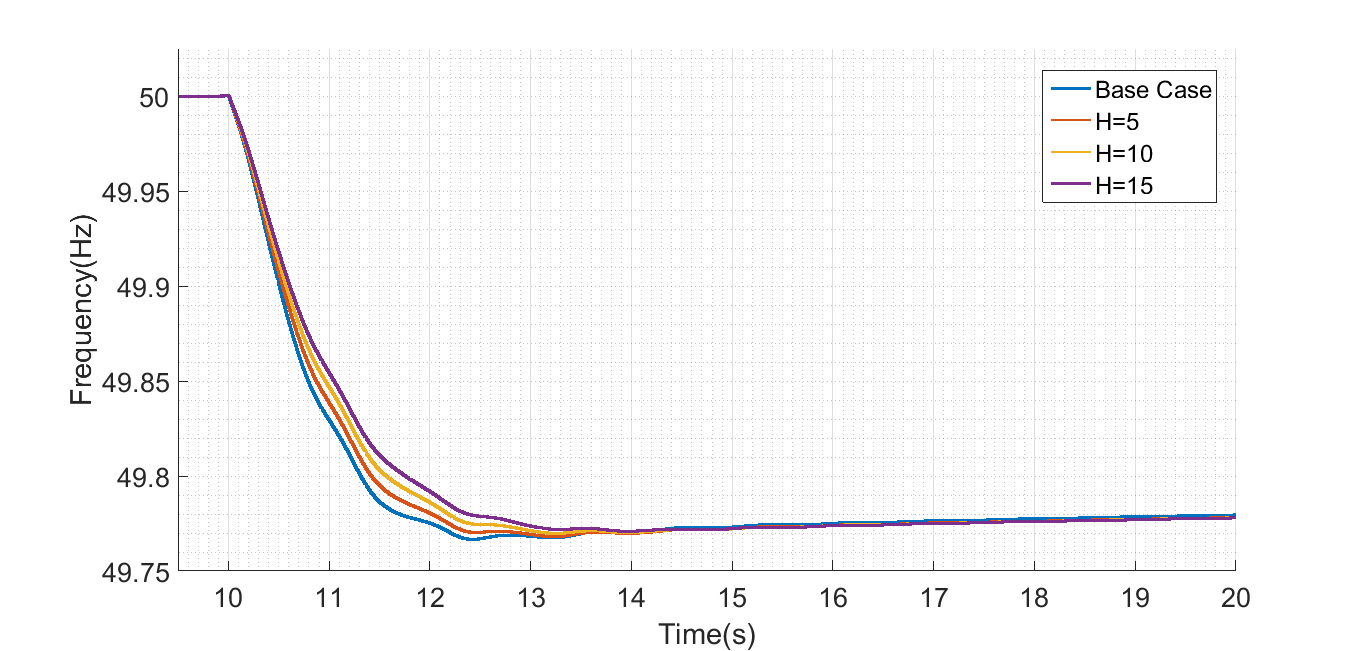
\includegraphics[width=0.9\linewidth]{case4_frequencies.png}
		\caption{Comparison of Frequencies}		
		\label{Case4_freq}
	\end{subfigure}
\vspace{0.1em} % here you can insert horizontal or vertical space
\begin{subfigure}{0.9\textwidth}
	\centering	
	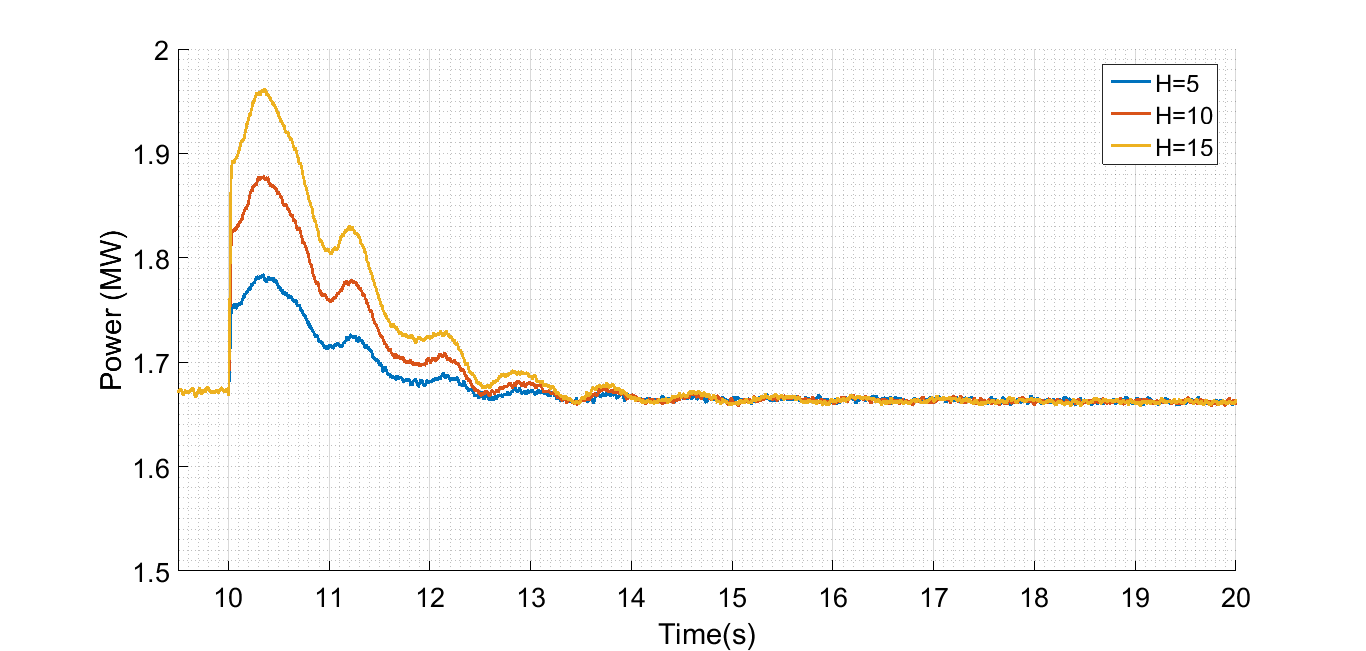
\includegraphics[width=0.9\linewidth]{case4_powers.png}
	\caption{Active Power Generations of the Wind Farms (wind speed=9m/s and n=1490rpm)}
	\label{Case4_power}	
\end{subfigure}
	\vspace{0.1em} % here you can insert horizontal or vertical space
	\begin{subfigure}{0.9\textwidth}
		\centering	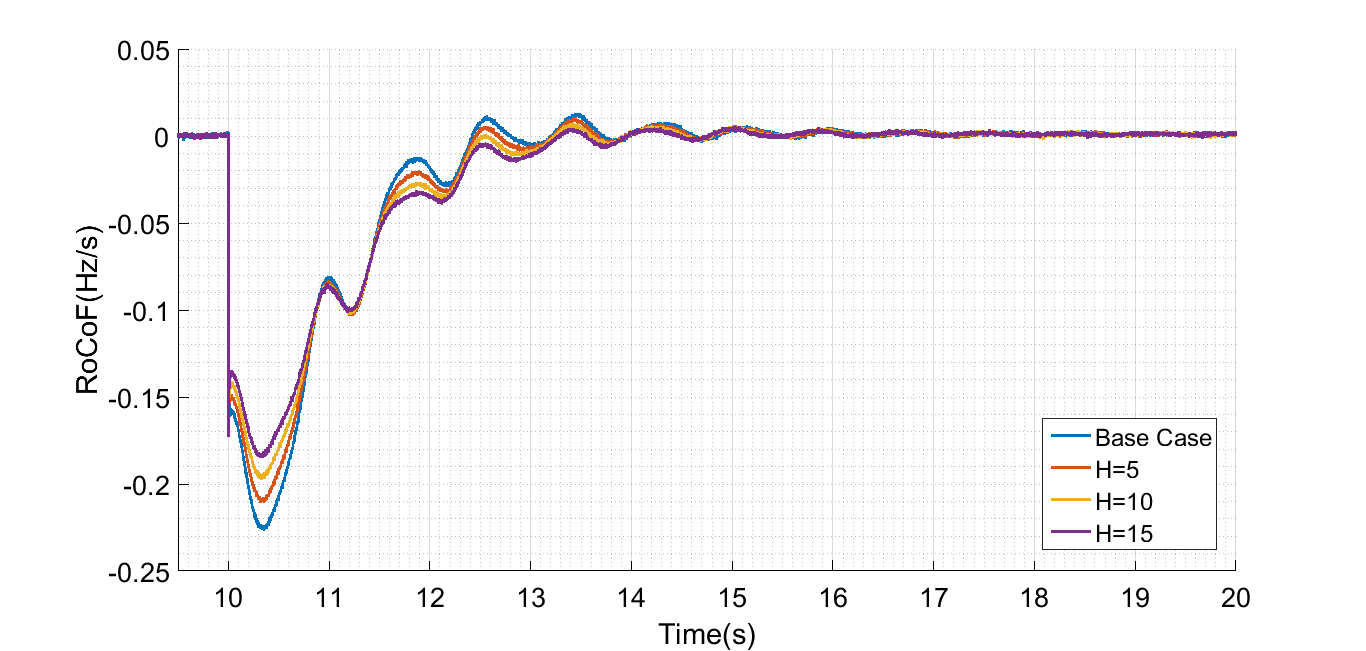
\includegraphics[width=0.9\linewidth]{case4_rocof.png}
		\caption{Comparison of RoCoFs}
		\label{Case4_rocof}	
	\end{subfigure}
	\caption{Emulation of the Different Inertia Constants in the \%10 Renewable Generation Case}
\end{figure}

Since the modified case frequency response is almost the same with the base case, the synthetic inertia implementation is improved the system frequency response. In other words, the wind turbines are integrated to the system by emulating the synchronous generator behaviour. It should be noted that huge amount of kinetic energy up to 18 MJ exists in the wind turbine systems. That stored energy can be utilized with the synthetic inertia method in order to improve frequency dynamics of the system. \par
Emulation of synchronous generator behaviour is basically increasing the amount of active power depending on the RoCoF of the grid and the inertia constant to be emulated. Since the higher inertia constant requires higher active power increase, the inertia constants of 10s and 15s result in better frequency dynamics. The frequency nadir of the base case is slightly increased. \par
The effect of the synthetic inertia provision can also be observed in the system RoCoF values. Fig. \ref{Case4_rocof} shows that the base case experiences RoCoF up to 0.23Hz/s during the first second of the frequency disturbance. While the remaining cases is subjected to lower RoCoF at first (0.18-0.21Hz/s), the base case RoCoF is the lowest following seconds. Another observation is that all cases converges to the same steady state frequency due to the fact that inertial support affects the transient rather than the steady state values. The steady state frequency is dependent on the capacity of conventional synchronous generators and their droop constants. This is why the reduced inertia case steady state frequency is lower than that of 10\% renewable case. Due to the fact that the frequency nadir of the system is closed to the steady state frequency (the frequency where the decline in the frequency is arrested and stabilized), the improvement in the frequency nadir is small. The system frequency nadir would be improved significantly if the frequency nadir is significantly below the steady state frequency. 
\section{Reduced Inertia Case with Synthetic Inertia}
Reduced Inertia case frequency response for 10\% additional load connection is studied in the Section \ref{sec:kdecommissioned}. The System frequency experiences high RoCoF up to 0.25Hz/s and frequency nadir, 49.65Hz because of the removal of the generator-3. In this section, synthetic inertia method is again implemented in the wind farm with different inertia constants 5s, 10s and 15s. The resultant frequency responses are shown in the Fig. \ref{Case5_freq}. As in the 10\% renewable case, base case frequency response experiences steepest decline up to 0.25Hz/s meanwhile the maximum value of RoCoF decreases down to 0.19Hz/s. \par
The active power generations of the wind farm for the different inertia constants are given in Fig. \ref{Case5_power}. It should be noted that the active power of the wind turbine is proportional with the RoCoF that is also given in Fig. \ref{Case5_rocof}. Notice that inertia constant H=15s is also emulated. It is stated that conventional generator inertia constants lie between 2-9s \cite{Kundur}. Nonetheless, synchronous generators have constant kinetic energy in the nominal frequency. However, the kinetic energy stored in the turbine inertia fluctuates with the generator speed. Moreover, wind turbine is able to emulate different inertia constant as soon as it has the capacity to increase its power. Even with the inertia constant of 15s, the wind turbine is far away from its maximum allowable power for the wind speed 9m/s. However, the turbine inertia constant is limited with H=10s for the high wind speed operation. In this way, it is ensured that wind turbine is able to emulate the inertia constant H=10s independent of the wind speed. However, the turbine is under utilized for the low and medium wind speed ranges.\par
The comparison of the case properties are listed in Table \ref{casescomp}. 
\begin{figure}[h!]
	\centering
	\begin{subfigure}{0.9\textwidth} % width of right subfigure
		\centering	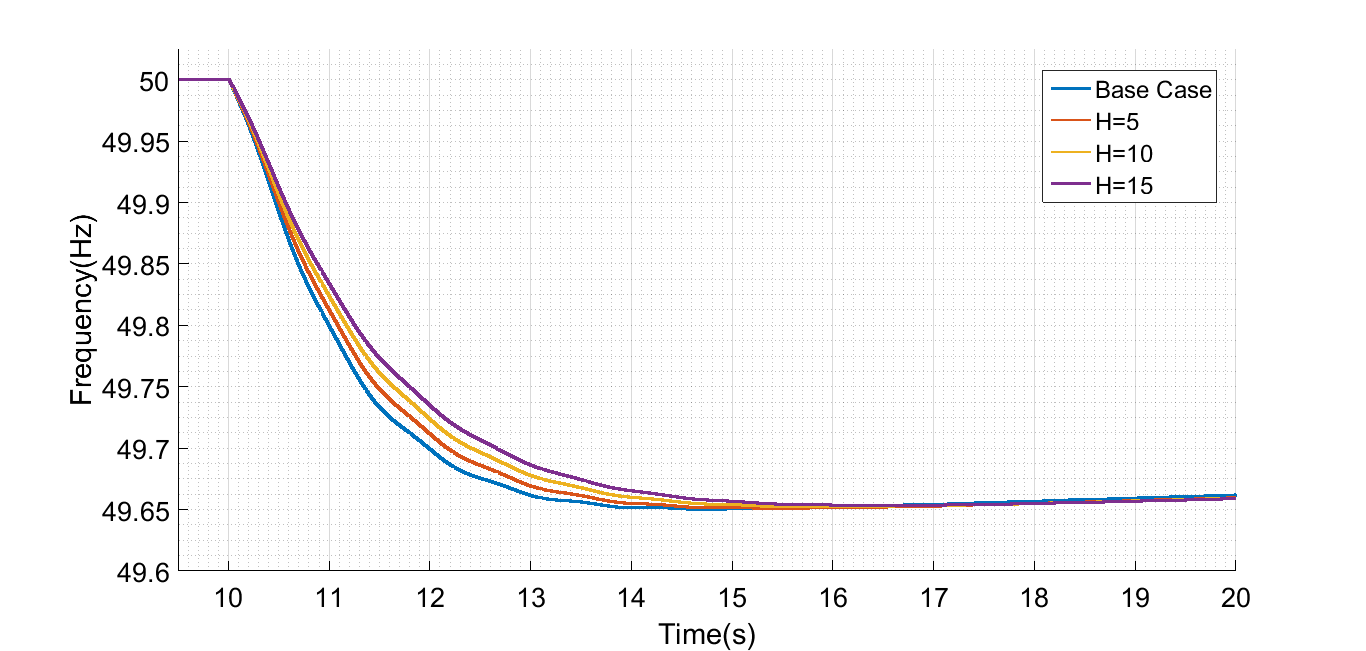
\includegraphics[width=0.9\linewidth]{case5_frequency.png}
		\caption{Comparison of Frequencies}		
		\label{Case5_freq}
	\end{subfigure}
	\vspace{0.1em} % here you can insert horizontal or vertical space
	\begin{subfigure}{0.9\textwidth}
		\centering	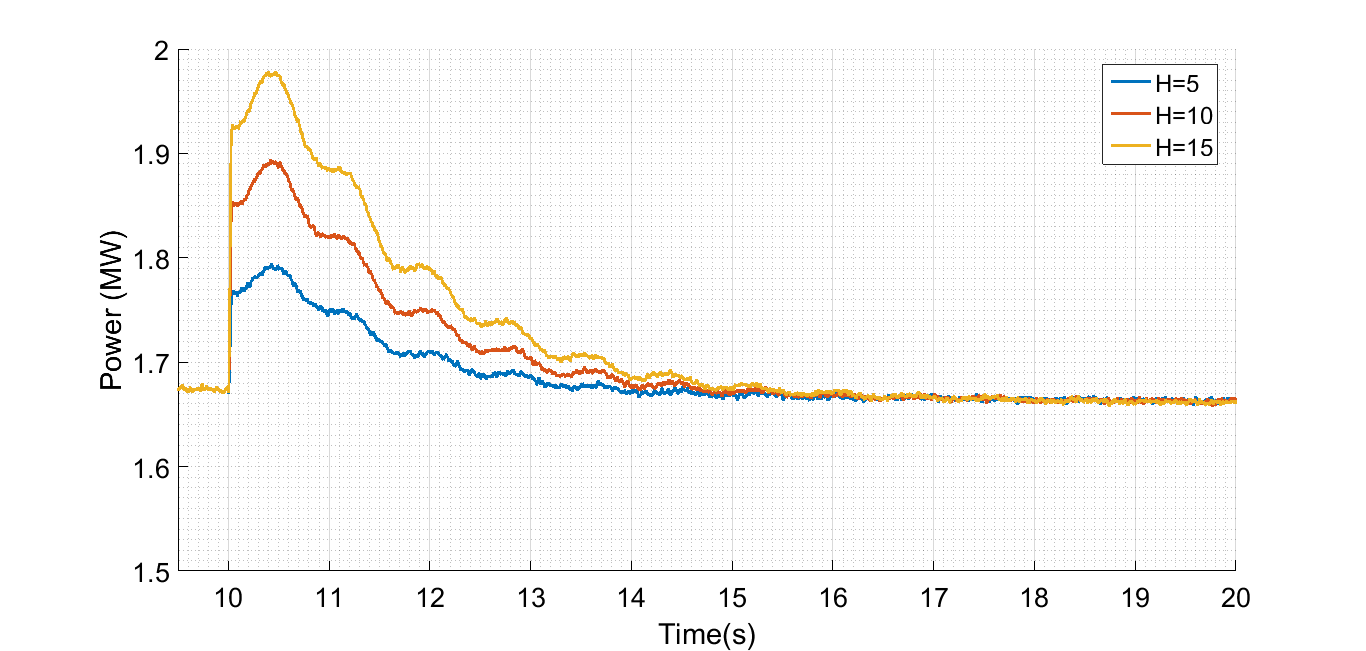
\includegraphics[width=0.9\linewidth]{case5_powers2.png}
		\caption{Active Power Generations of the Wind Farms (wind speed=9m/s and n=1490rpm)}
		\label{Case5_power}	
	\end{subfigure}
	\vspace{0.1em} % here you can insert horizontal or vertical space
	\begin{subfigure}{0.9\textwidth}
		\centering	
		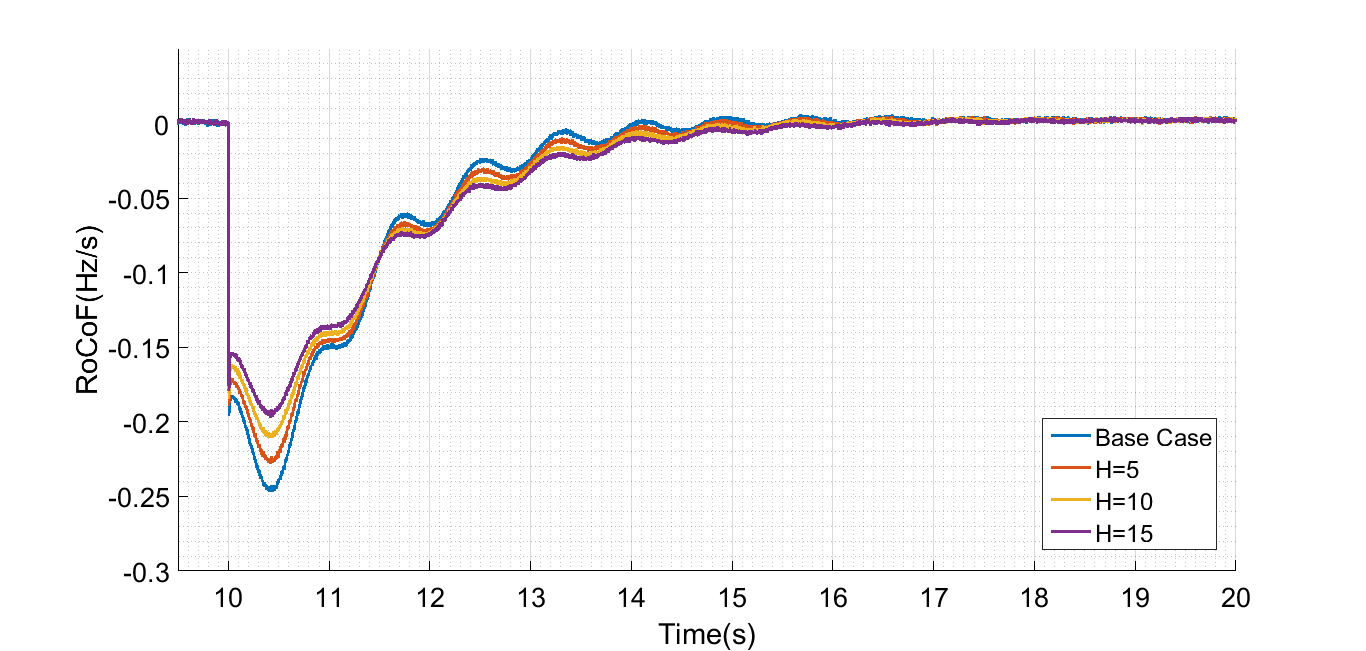
\includegraphics[width=0.9\linewidth]{case5_rocof.png}
		\caption{Comparison of RoCoFs}
		\label{Case5_rocof}	
	\end{subfigure}
	\caption{Emulation of the Different Inertia Constants in the Reduced Inertia Case}
\end{figure}
% Please add the following required packages to your document preamble:
% \usepackage{graphicx}
\begin{table}[h!]
	\centering
	\resizebox{\textwidth}{!}{%
		\begin{tabular}{|c|c|c|c|c|c|}
			\hline
			& \multicolumn{3}{c|}{\begin{tabular}[c]{@{}c@{}}Without Synthetic\\ Inertia Implementation\end{tabular}}                                                                                         & \multicolumn{2}{c|}{\begin{tabular}[c]{@{}c@{}}With Synthetic Inertia\\ (H=10s)\end{tabular}}                                              \\ \cline{2-6} 
			& \begin{tabular}[c]{@{}c@{}}Base\\ Case\end{tabular} & \begin{tabular}[c]{@{}c@{}}10\% Renewable\\ Generation Case\end{tabular} & \begin{tabular}[c]{@{}c@{}}Reduced Inertia\\ Case\end{tabular} & \begin{tabular}[c]{@{}c@{}}10\% Renewable\\ Generation Case\end{tabular} & \begin{tabular}[c]{@{}c@{}}Reduced Inertia \\ Case\end{tabular} \\ \hline
			\begin{tabular}[c]{@{}c@{}}Stored Kinetic\\  Energy\end{tabular}          & 3.3                                                 & 3.6                                                                      & 3.3                                                            & 3.6                                                                      & 3.3                                                             \\ \hline
			\begin{tabular}[c]{@{}c@{}}Effective\\ Kinetic Energy\\ (GJ)\end{tabular} & 3.3                                                 & 3.3                                                                      & 3                                                              & 3.9                                                                      & 3.6                                                             \\ \hline
			\begin{tabular}[c]{@{}c@{}}Maximum\\ RoCoF\\ (Hz/s)\end{tabular}          & 0.23                                                & 0.23                                                                     & 0.25                                                           & 0.19                                                                     & 0.21                                                            \\ \hline
			\begin{tabular}[c]{@{}c@{}}Frequency\\  Nadir\\ (Hz)\end{tabular}         & 49.77                                               & 49.77                                                                    & 49.65                                                          & 49.77                                                                    & 49.65                                                           \\ \hline
		\end{tabular}%
	}
	\caption{Comparison of the Case Properties}
	\label{casescomp}
\end{table}
\section{Comparison of the Synthetic Inertia and Fast Inertial Support}
In the Chapter \ref{chp:4}, it is shown that the wind turbines have sufficient capacity in order to increase its active power. For medium and high wind speed cases, increase up to 48\% can be achieved. This capacity in the wind turbine is utilized in Chapter \ref{chp:4} for the fast inertial support which is the fast release of active power from energy generating unit. The exaggerated inertial supports are studied to observe the turbine internal dynamics. Besides, the fast inertial support is studied for 10\% increase in the active power in different support durations.\par
In this section, the fast inertial support will be compared with the inertial support that is proportional to grid RoCoF. In other words, increasing active power by a defined percentage will be compared to a rise in the active power proportional to RoCoF. For this reason, the same frequency disturbance is tested on the reduced inertia case, the case where inertia constant of 10s is emulated and also the one with fast inertial support with 5\% increased power by 5 seconds. The inertia constant is selected as 10s since it is applicable to whole wind speed range. The fast inertial support with 5\% active power increase is selected such that the same amount energy will be extracted from wind turbine during the 5 seconds following the disturbance. Fig. \ref{Comp_power} shows the variation of the active power. It should be underlined that the active power of the inertia emulated case is increased proportional to the RoCoF. Therefore, it declines as the RoCoF declines. Therefore, in the other half of the support time, it is below of the fast inertial support case. This phenomena can be clearly observed in the frequency response. Nonetheless, the active power of the fast inertial support is the same during the support.\par
\begin{figure}[h]
	\centering
	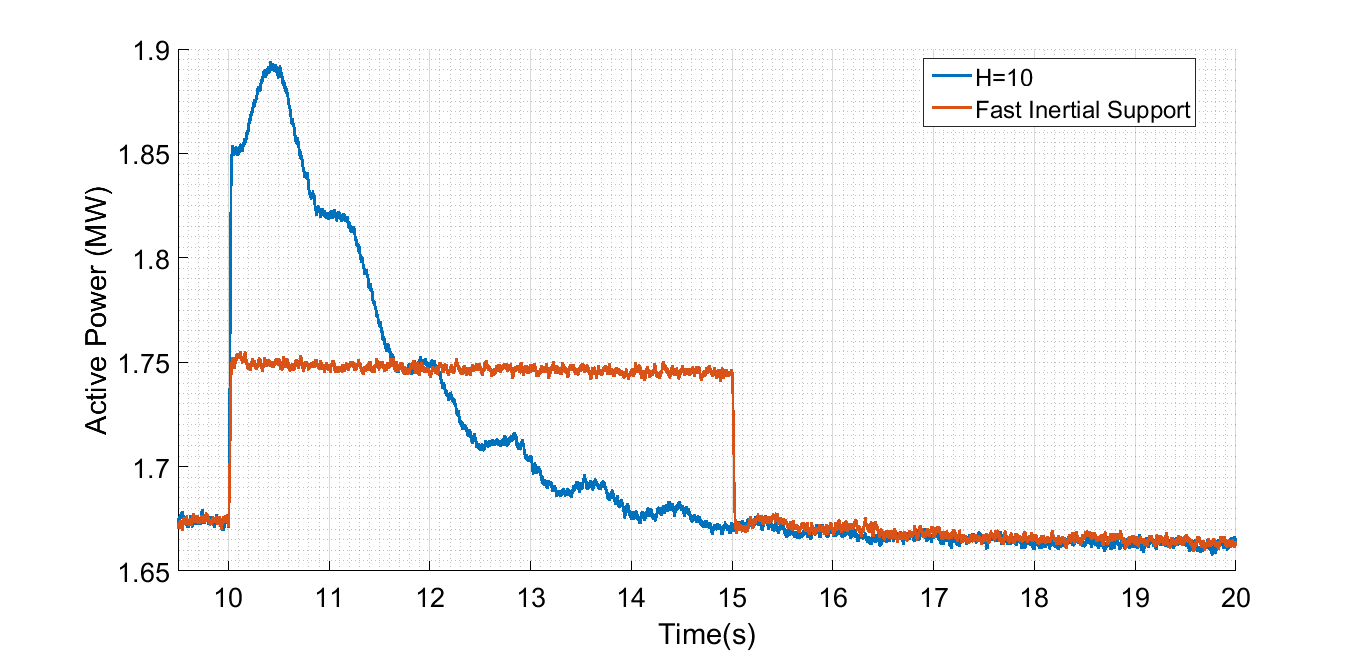
\includegraphics[width=0.9\linewidth]{comparison_power.png}
	\caption{Comparison of the Frequency Responses for the Base, Fast Inertial Support and Synthetic Inertia Cases}
	\label{Comp_power}
\end{figure}
The frequency response of these three cases is shown in Fig. \ref{Comp_freq}. It is obvious that the base case frequency response has the poorest transient frequency. Besides, the synthetic inertia implemented case has the best transient behaviour for the very first seconds. Nonetheless, the fast inertial support case first converges to higher steady state frequency until the end of the support period. However, as soon as the support ends, the sharp decrease in the active power results a second dip in the frequency. The decrease in the active power can be considered as a second load connection to system. Therefore, the frequency is exposed to a second decrease at the end of support period in fast inertial support implementation. In contrary, the synthetic inertia case active power is decreased down to lower values as the RoCoF is positive. Than means that the recovery process is already started inside the support. Hence, the secondary dip is not observed in this case. \par
\begin{figure}[h!]
	\centering
	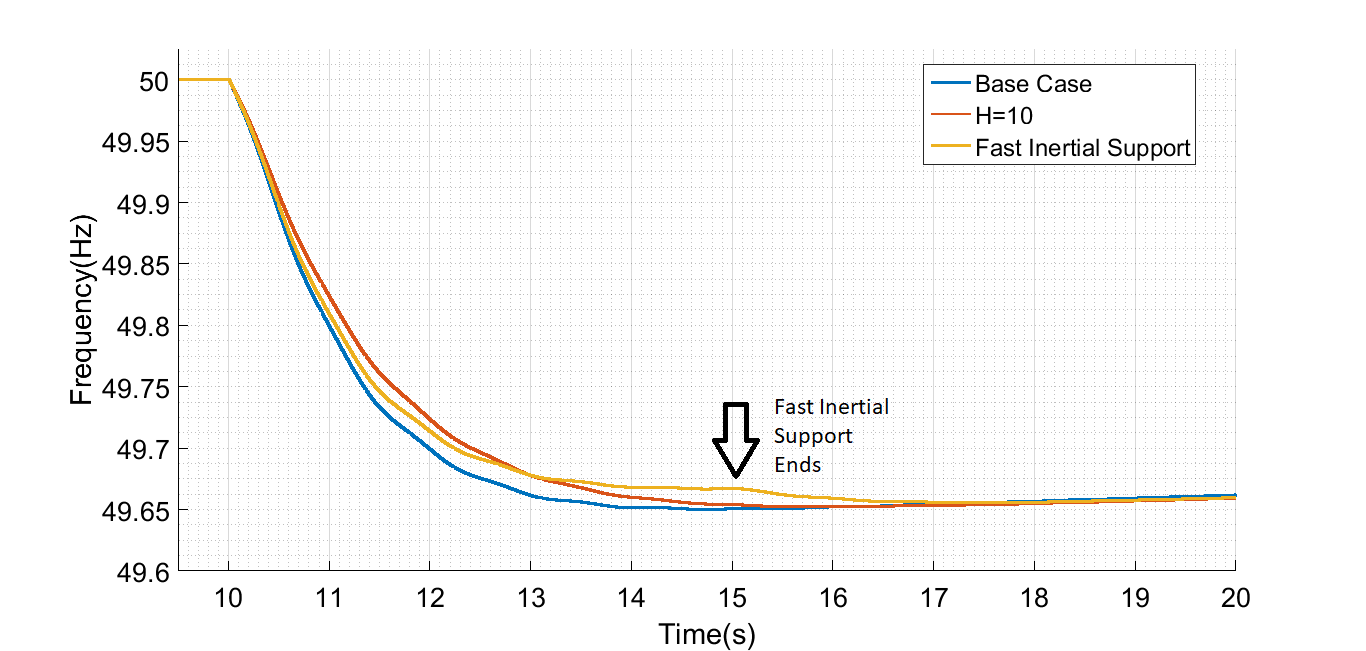
\includegraphics[width=0.95\linewidth]{comparison_freq.png}
	\caption{Comparison of the Active Power Increase in Fast Inertial Support Case and Synthetic Inertia Case}
	\label{Comp_freq}
\end{figure}
Finally, it should be noted that the energy extracted from wind turbine in the first 4 seconds are the same for both methods. However, synthetic inertia support utilizes that energy better by distributing the energy according to the RoCoF. The maximum value of the RoCOF in the Reduced Inertia case is 0.25Hz/s. The fast inertial support decreases the RoCoF value down to 0.23Hz/s. Nonetheless, maximum value of the RoCoF decreases to 0.21Hz/s with the synthetic inertia implementation thanks to the active power increase according to the RoCoF. The maximum value of the RoCoF is crucial especially for the RoCoF relays. Even though the frequency nadir in the system is not increased significantly, the limitation of the RoCoF value is important for the successful operation of the system. If one more outage due to the RoCoF protection of the generator occurs in the system, the cascading generator trip might end up with the system blackout. Therefore, the synthetic inertia implementation is important for weak power systems with high wind penetration.
\section{Conclusion}
In this chapter, it is shown that the wind turbine is able to emulate high inertia constants up to 32.9s. In the low and medium speed range, the turbine converter has capacity to increase the power by significant amounts such as 1.3MW. Nonetheless, the turbine converter is not available for the increase in the active power especially in high wind speeds. Therefore, the inertia constant that can be emulated inside the whole wind speed range is found out to be 10s. \par
The provision of inertial support that is proportional to grid RoCoF is more advantageous than that of fast inertial support. First of all, the grid frequency is not subjected to a second frequency dip since the support power goes below the pre-disturbance power according to the RoCoF. In contrary, the step decrease at the end of support duration creates another frequency disturbance in the fast inertial support. Therefore, synthetic inertia implementation is more appropriate for weak power systems compared to fast inertia support since it deteriorates the stability of the weak power systems. Another advantage of the synthetic inertia implementation is the provision of additional power that is proportional to grid RoCoF. In this way, the turbine contributes the grid stability depending on the requirement of the power grid. Therefore, the synthetic inertia implementation is better shaped fast inertial support.\par
Wind turbines can contribute to the grid frequency stability by emulating inertia constants. A variety of inertia constants can be emulated by wind turbine inside the low and medium speed ranges. However, the high wind speed scenario limits the active power increase and the inertia constant to be emulated. Therefore, inertia constant H=10s is appropriate for the whole wind speed range. By considering the inertia constant H=10s, the contribution to grid inertia can be calculated. \par
The installed wind energy capacity of the Turkey has reached 7012MW on the July 2018 \cite{July2018}. In the Turkish market, 97\% of the installed wind turbines belongs to Nordex, Enercon, Vestas, GE, Siemens and Gamesa. The wind turbine topology used by Nordex is DFIG which is connected to grid by partial scale power converter (PSPC) meanwhile the models of Enercon are connected to grid by full-scale power converter (FSPC). Besides, Vestas and GE uses both DFIG or PMSG topologies. By considering the wind turbine models inside the wind farms in Turkey, the share of the wind turbines that are connected to grid with FSPC is found as 54\%. The share of the wind turbines with FSPC can be used to estimate the energy produced by this category. \par
The aggregated inertia constant of the electricity network depends on the generation variety. In other words, the grid aggregated inertia changes according to the share of the conventional generators and the share of renewable energy in the total energy production. Therefore, it is a function of the stored kinetic energy and the total generated power. The variation of the power generation between 01 Jan. 2018 and 31 Dec. 2018 is given in the Fig. \ref{overallprod} according to the data shared by TEİAŞ Transparency Platform. The highest generation occurs on 03 Aug. 2018 as 45923MW and the lowest generation is on 16 Jun. 2018. \par
\begin{figure}[h!]
	\centering
	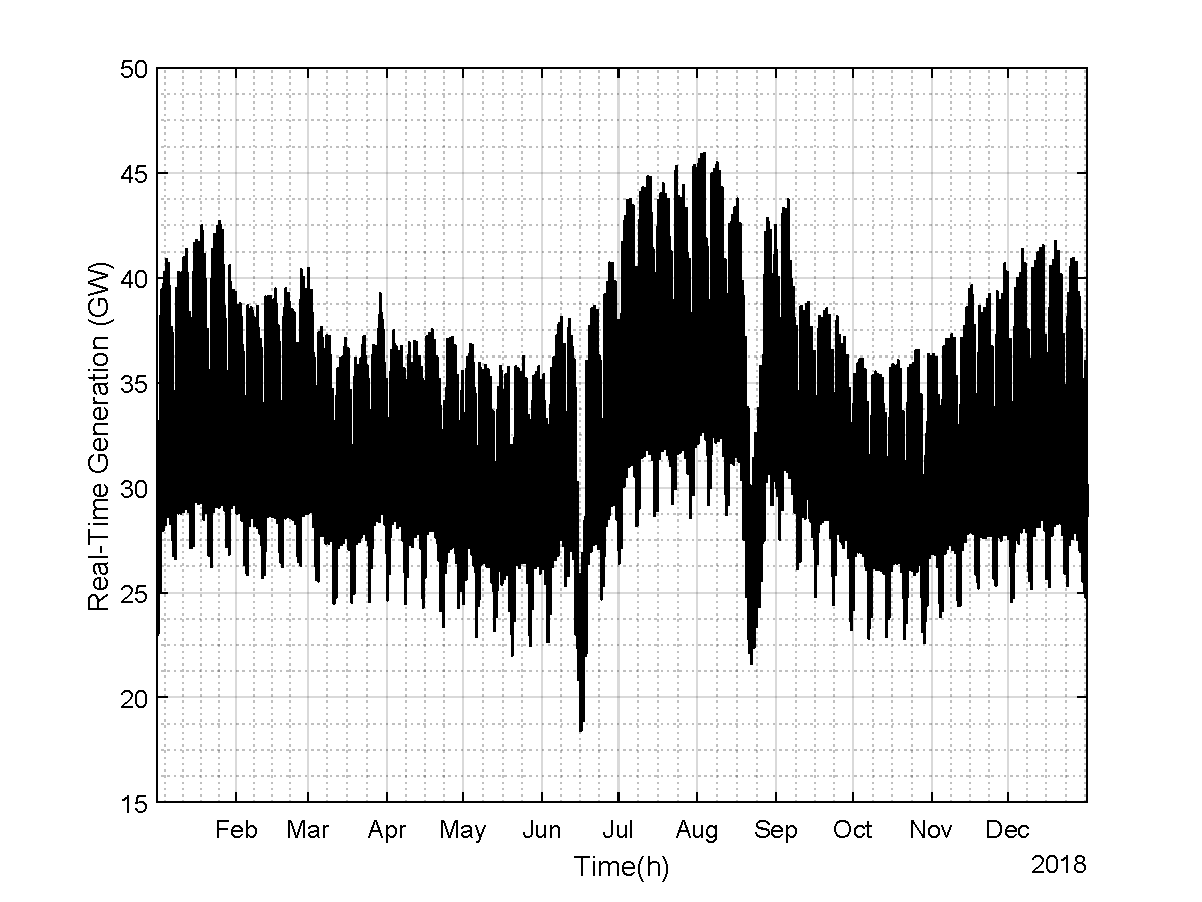
\includegraphics[width=0.9\linewidth]{overallproduction.pdf}
	\caption{Variation of the Energy Production between 01 Jan. 2018 and 31 Dec. 2018 (hourly basis)}
	\label{overallprod}
\end{figure}
The  inertia constants of conventional synchronous generator vary between 2-9s \cite{Kundur} as stated in the previous chapters. The stored kinetic energy in the electricity network is estimated by assuming inertia constant H=5s for conventional generators and zero inertia constant for wind and solar energy generation. Due to the absence of the inertial contribution from wind and solar energy systems, the aggregated inertia constant goes below 5s. The aggregated inertia constant deviates from 5s with the increase in the wind and solar generation. The variation of the aggregated inertia constant is depicted in Fig. \ref{overallinertia}. The minimum and maximum of aggregated inertia is 3.97s and 4.99s respectively.\par
\begin{figure}[h!]
	\centering
	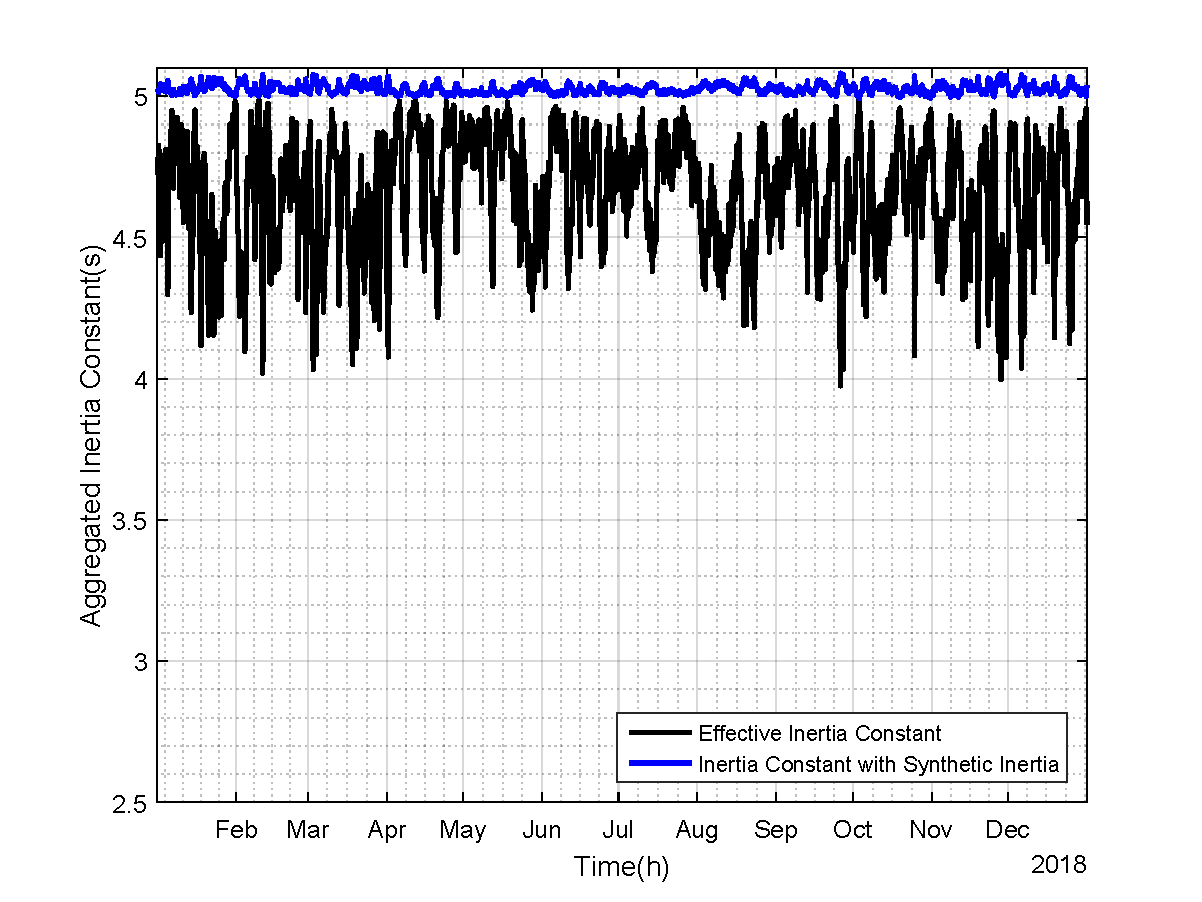
\includegraphics[width=0.9\linewidth]{agg_inertia.pdf}
	\caption{Variation of the Aggregated Inertia Constant between 01 Jan 2018 and 31 Dec. 2018 (hourly basis)}
	\label{overallinertia}
\end{figure}
The grid aggregated inertia can be increased by the synthetic implementation in the wind turbines with FSPC. In order to estimate the system inertia with the synthetic inertia implementation, all wind turbines with back-to-back converter are assumed to be able to provide inertial support with the inertia constant H=10s. Moreover, it is assumed that the generated wind power is distributed homogeneously inside each wind farm. In this way, the generation from FSPC wind turbines can be assumed as 54\% of total wind generation. According to these assumptions, grid aggregated inertia constant is calculated and presented in Fig. \ref{overallinertia}. In this case, the minimum and maximum values of the inertia constant is found out to be 4.99s and 5.08s. \par
\begin{table}[]
	\centering
	\resizebox{\textwidth}{!}{%
		\begin{tabular}{|c|c|c|c|c|c|}
			\hline
			\multicolumn{3}{|c|}{Existing  System} & \multicolumn{3}{c|}{\begin{tabular}[c]{@{}c@{}}Inertial\\   Support Implementation (H=10s)\end{tabular}} \\ \hline
			& \begin{tabular}[c]{@{}c@{}}Minimum Inertia\\ H=3.97s\end{tabular} & \begin{tabular}[c]{@{}c@{}}Maximum Inertia\\ H=4.99s\end{tabular} &  & \begin{tabular}[c]{@{}c@{}}Minimum Inertia\\ H=4.99s\end{tabular} & \begin{tabular}[c]{@{}c@{}}Maximum Inertia\\ H=5.08s\end{tabular} \\ \hline
			Date & \begin{tabular}[c]{@{}c@{}}26/09/2018 \\ 03:00\end{tabular} & \begin{tabular}[c]{@{}c@{}}12/04/2018\\ 09:00\end{tabular} & Date & \begin{tabular}[c]{@{}c@{}}03/10/2018\\ 10:00\end{tabular} & \begin{tabular}[c]{@{}c@{}}26/09/2018\\ 03:00\end{tabular} \\
			\begin{tabular}[c]{@{}c@{}}Total \\ Generation\\ (MW)\end{tabular} & 27495.5 & 34828.4 & \begin{tabular}[c]{@{}c@{}}Total \\ Generation\\ (MW)\end{tabular} & 33552.0 & 27495.5 \\
			\begin{tabular}[c]{@{}c@{}}Wind (FSPC)\\ (MW)\end{tabular} & 3045.4 & 37.9 & \begin{tabular}[c]{@{}c@{}}Generation\\ (MW)\end{tabular} & 26.7 & 3045.4 \\
			\begin{tabular}[c]{@{}c@{}}Wind (Other)\\ (MW)\end{tabular} & 2594.2 & 32.3 & \begin{tabular}[c]{@{}c@{}}Wind (Other)\\ (MW)\end{tabular} & 22.8 & 2594.2 \\
			\begin{tabular}[c]{@{}c@{}}Solar\\ (MW)\end{tabular} & 0.0 & 11.7 & \begin{tabular}[c]{@{}c@{}}Solar \\ (MW)\end{tabular} & 56.4 & 0.0 \\
			\begin{tabular}[c]{@{}c@{}}Other\\ (MW)\end{tabular} & 21772.9 & 34639.5 & \begin{tabular}[c]{@{}c@{}}Other\\ (MW)\end{tabular} & 33446.1 & 21772.9 \\ \hline
		\end{tabular}%
	}
	\caption{Contribution of the Synthetic Inertia Implementation to System Aggregated Inertia based on 2018 Generation Data}
\label{contribution}
\end{table}
The network details of the inertia constant extremes are listed in Table. \ref{contribution}. The existing system inertia constant deviates according to the share of the generation. The inertia constant decreases down to 3.97s that is the worst case scenario in the system. The reason of the decrease is the high wind generation profile. Nonetheless, best improvement in the aggregated inertia constant is achieved with the same scenario. This means that the existing wind turbines with FSPC are able to compensate the deterioration caused by other wind turbine technologies (DFIG and other).